

    For all the examples we show here, we only show the ordering relations that are important to observe. 
    Putting all the relations among different events in the example will result in confusion, hence we avoid them. 

    \paragraph{Reads to same memory where $e$ is of type $sc$ while $d$ is of either $uo/sc$}

        The following example illustrates when reordering two reads to $x$ as per the specification of their access orders and range results in an observable behavior disallowed.
        Figure~\ref{reord_counter:example1(a)} shows an example of a candidate(left) along with with its candidate execution(right) where the case of outcome in the red box is not possible. 
        \begin{figure}[H]
            \centering
            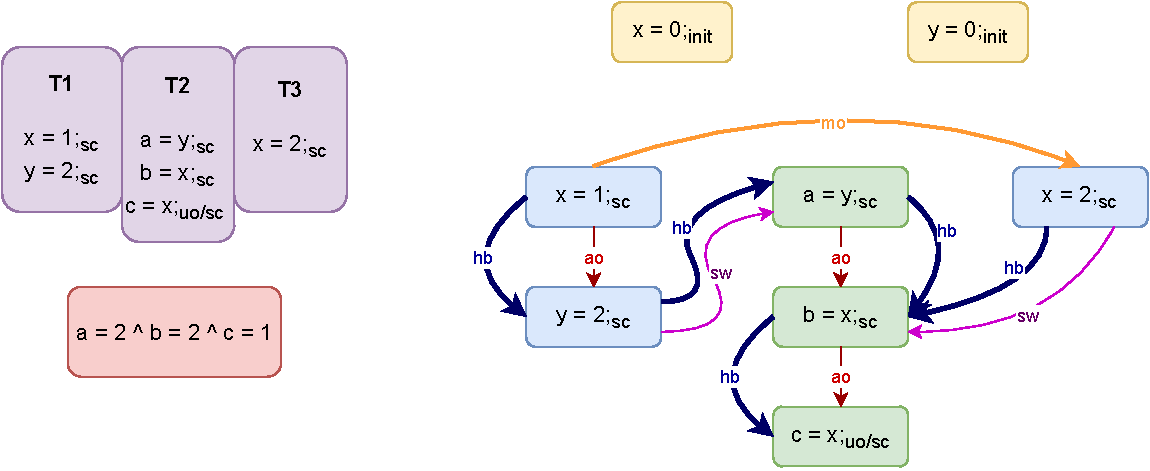
\includegraphics[scale=0.7]{7.CounterExamples/ReorderingCandidate/Example0(Rsc-Ruo,sc).pdf}
            \caption{Case where $a = 2, b = 2, c = 1$ is invalid due to Sequentially Consistent Atomics}
            \label{reord_counter:example1(a)}
        \end{figure}
        
        Observations:
        \begin{itemize}
            \item We can infer from the Candidate Execution that $\reln{x=1;_{sc}}{hb}{b=x;_{sc}}$.
            \item Because $\reln{\{x=2;_{sc}\}}{sw}{\{b=x;_{sc}\}}$, this means the read value of $b$ is $2$.
            \item From the above two, we can infer $\reln{\{x=2;_{sc}\}}{mo}{\{x=2;_{sc}\}}$.
            \item We can then also infer that $\reln{\{x=1;_{sc}\}}{hb}{\{c=x;_{uo/sc}\}}$ and $\reln{\{x=2;_{sc}\}}{hb}{\{b=x;_{uo/sc}\}}$.
            \item By Axiom \ref{SeqCsAt} pattern 1 and 3, the read value for $c$ cannot be $1$.
        \end{itemize}

        Figure~\ref{reord_counter:example1(b)} shows the Candidate(right) after reordering the two reads in $T2$ along with its candidate execution(left) where the same case of reads(orange box) is possible. 
        \begin{figure}[H]
            \centering
            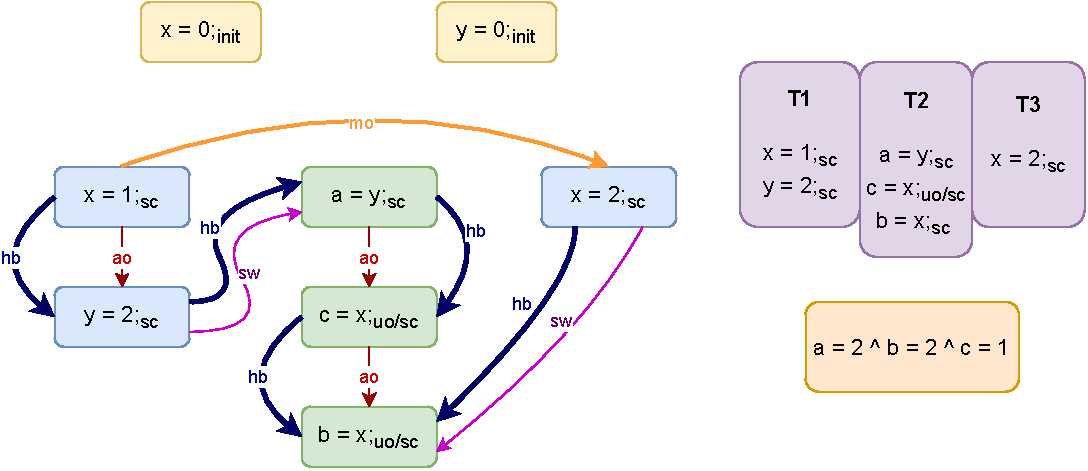
\includegraphics[scale=0.7]{7.CounterExamples/ReorderingCandidate/Example0R(Rsc-Ruo,sc).pdf}
            \caption{Case where the reads are reordered and $a = 2 , b = 2, c = 1$ is valid.}
            \label{reord_counter:example1(b)}
        \end{figure}

        Observations
        \begin{itemize}
            \item We can infer from the Candidate Execution that $\reln{\{x=1;_{sc}\}}{hb}{\{c=x;_{uo/sc}\}}$.
            \item No Axiom has restrictions on $\stck{_{rf}}$ between the above two events.
            \item Hence, the read value of $c$ can be $1$.
            \item Further, the memory order is not inferred yet\footnotemark, hence, the read value for $b$ can be $2$.
            \item Hence the reordering of the two reads is invalid. 
        \end{itemize}

        \footnotetext{Note that if the memory order was reversed in the original candidate execution, Axiom \ref{SeqCsAt} would restrict the value of $b$ to be $1$. Since this is not possible due to the synchronized relation established, it must be the case that $x=1$ is memory ordered before $x=2$.}
        
%---------------------------------------------------------------------------------------------------------------------------------------
    
    \paragraph{A Read $e$ of type $sc$ followed by a Write of either $uo/sc$}
        
        Figure~\ref{reord_counter:example2(a)} shows an example of a candidate(left) along with with its candidate execution(right) where the case of outcome in the red box is not possible. 
        \begin{figure}[H]
            \centering
            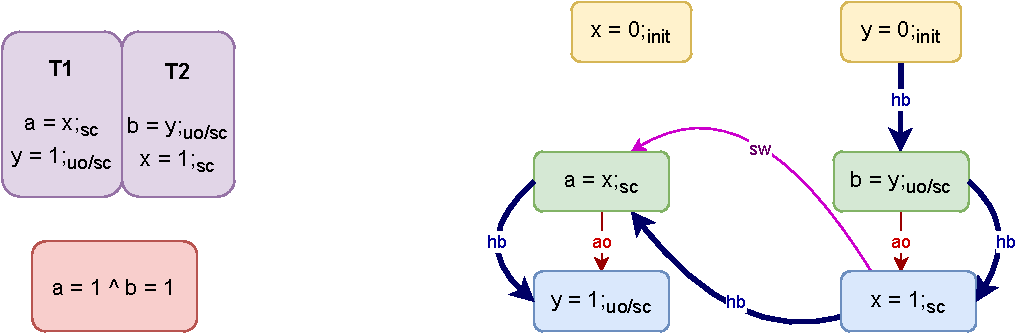
\includegraphics[scale=0.7]{7.CounterExamples/ReorderingCandidate/Example3(Rsc-Wuo,sc).pdf}
            \caption{Case where $a = 1, b = 1$ is invalid due to Coherent Reads.}
            \label{reord_counter:example2(a)}
        \end{figure}

        Observations:
        \begin{itemize}
            \item From the Candidate Execution, we can infer $\reln{\{b=y_{uo/sc}\}}{hb}{\{y=1_{uo/sc}\}}$
            \item By Axiom \ref{CoRe}, $b$ cannot read the value of $1$ as $y$. 
            \item This inference was due to $\reln{\{x=1_{sc}\}}{hb}{\{a=x{sc}\}}$
        \end{itemize}

        Figure~\ref{reord_counter:example2(b)} shows the Candidate after reordering(right) a read and write in $T1$ along with its candidate execution(left) where the same case of reads(orange box) is possible. 
        \begin{figure}[H]
            \centering
            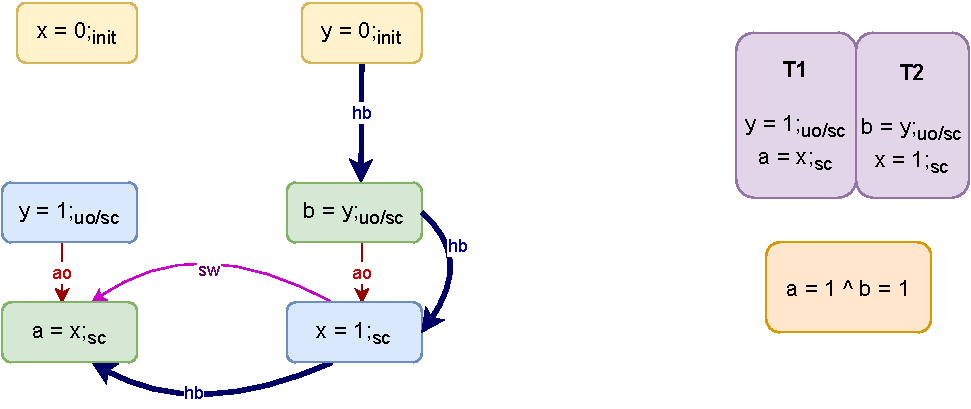
\includegraphics[scale=0.7]{7.CounterExamples/ReorderingCandidate/Example3R(Rsc-Wuo,sc).pdf}
            \caption{Case where events of T1 are reordered, resulting in $a = 1, b = 1$ to be valid.}
            \label{reord_counter:example2(b)}
        \end{figure}
        
        Observations:
        \begin{itemize}
            \item From the Candidate Execution, we can infer $\neg\reln{\{b=y_{uo/sc}\}}{hb}{\{y=1_{uo/sc}\}}$
            \item Since there is no $\stck{_{hb}}$ relation among the above two events, $b$ can read the value of $y$ as $1$.
        \end{itemize}

%--------------------------------------------------------------------------------------------------------------------------------------        
    \paragraph{A Read $e$ of type $uo$ followed by a write $d$ of type $sc$}

        For this we can use the same example in Figure~\ref{reord_counter:example2(a)} where we just reorder $T2$'s events.
        We leave justifying the new observable behavior introduced as an exercise for the reader.
    
%---------------------------------------------------------------------------------------------------------------------------------------
        
    \paragraph{A Write $e$ followed by a Read $d$ both of type $sc$}
        
        A counter example for this is different. 
        It is not the Observable Behavior we are concerned with that is introduced, but that which is allowed but creates a $\stck{_{hb}}$ cycle. 
        Figure~\ref{reord_counter:example3(a)} is one such example with its Candidate and Corresponding Candidate Execution in question:
        \begin{figure}[H]
            \centering
            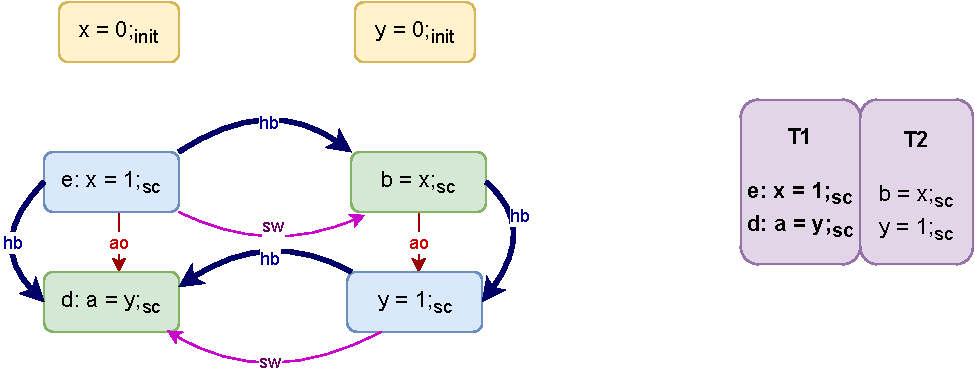
\includegraphics[scale=0.7]{7.CounterExamples/ReorderingCandidate/Example5(Wsc-Rsc).pdf}
            \caption{Case where $a = 1, b = 1$ is valid and no happens-before cycles}
            \label{reord_counter:example3(a)}
        \end{figure}

        Figure~\ref{reord_counter:example3(b)} shows the Candidate after reordering(right) the two events in $T1$, which makes the same candidate execution(right) as above contain a happens-before cycle:
        \begin{figure}[H]
            \centering
            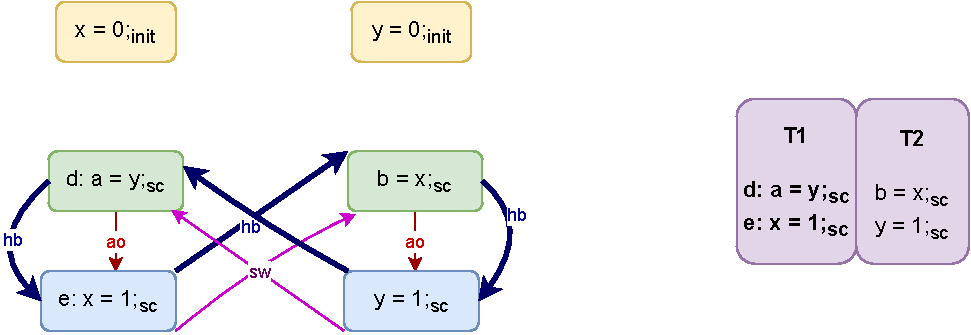
\includegraphics[scale=0.7]{7.CounterExamples/ReorderingCandidate/Example5R(Wsc-Rsc).pdf}
            \caption{Case where $a = 1, b = 1$ is creates a happens-before cycle}
            \label{reord_counter:example3(b)}
        \end{figure}

        Observation:
        \begin{itemize}
            \item From the read values we can infer that the Candidate Execution should have $\reln{\{x=1_{sc}\}}{hb}{\{a=x_{sc}\}}$ and $\reln{\{y=1_{sc}\}}{hb}{\{a=y_{sc}\}}$.
            \item The above relations create the cycle $\reln{\{a=y_{sc}\}}{hb}{\reln{\{x=1_{sc}\}}{hb}{\reln{\{a=x_{sc}\}}{hb}{\reln{\{y=1_{sc}\}}{hb}{\{a=y_{sc}\}}}}}$.
            \item This execution is invalid. 
        \end{itemize}

        One might think that simply discarding the above Candidate execution would do. 
        But this would mean discarding such $\stck{_{hb}}$ relations, which would require more information to infer which relations are going to create such cycles and which are not. 
        In practice a cycle may span several events from different threads.
        Since we place no assumptions on these relations, but that any happens-before relation other than the one we remove explicitly be reordering are all preserved. 
        Hence, the following reordered program outcome is something we do not risk to allow.

%---------------------------------------------------------------------------------------------------------------------------------------

    \paragraph{A Write $e$ of type $uo/sc$ followed by a Write $d$ of type $sc$}
        
        Figure~\ref{reord_counter:example4(a)} shows an example of a candidate(left) along with with its candidate execution(right) where the case of outcome in the red box is not possible. 
        \begin{figure}[H]
            \centering
            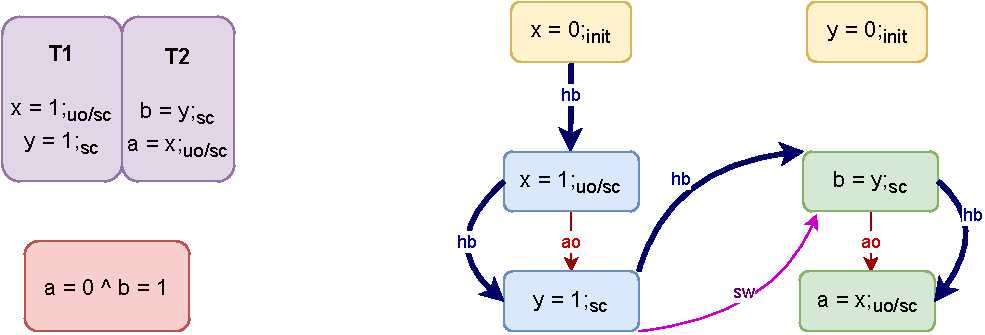
\includegraphics[scale=0.7]{7.CounterExamples/ReorderingCandidate/Example7(Wuo,sc-Wsc).pdf}
            \caption{Case where $a = 0, b = 1$ is invalid due to Coherent Reads.}
            \label{reord_counter:example4(a)}
        \end{figure}
        
        Observations:
        \begin{itemize}
            \item From the Candidate Execution, we can infer $\reln{\{x=0_{init}\}}{hb}{\reln{\{x=1_{uo/sc}\}}{hb}{\{a=x_{uo/sc}\}}}$
            \item By Axiom \ref{CoRe}, the read of $a$ cannot have the value of $x$ read as $0$. 
            \item This inference was due to $\reln{\{y=1_{sc}\}}{hb}{\{b=y_{sc}\}}$.
        \end{itemize}

        Figure~\ref{reord_counter:example4(b)} shows the Candidate after reordering(right) the two writes in $T1$ along with its candidate execution(left) where the same case of reads(orange box) is possible. 
        \begin{figure}[H]
            \centering
            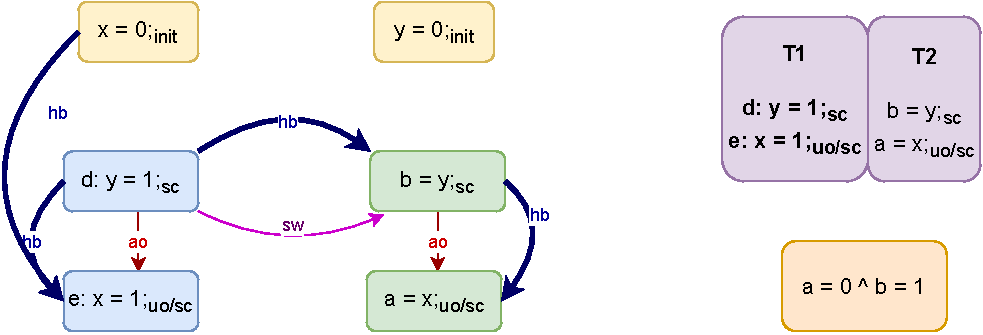
\includegraphics[scale=0.7]{7.CounterExamples/ReorderingCandidate/Example7R(Wuo,sc-Wsc).pdf}
            \caption{Case where events of T1 are reordered, resulting in $a = 0,  b = 1$ to be valid.}
            \label{reord_counter:example4(b)}
        \end{figure}
        
        Observations:
        \begin{itemize}
            \item From the Candidate Execution, we can infer $\neg\reln{\{x=1_{uo/sc}\}}{hb}{\{a=x_{uo/sc}\}}$
            \item There is no pattern that the Axioms restrict, thus validating $x$ to be read as $0$ by $a$. 
        \end{itemize}